% title: Data flow through two IR equations
% description: The runtime topic passes through two concat equations to produce the output. Each equation also takes a literal string. The intermediate value prompt connects the equations.
\documentclass[tikz,border=5pt]{standalone}
\usetikzlibrary{arrows.meta,calc,shapes.geometric}
\definecolor{numeric}{HTML}{4477AA}
\definecolor{textual}{HTML}{AA4499}

\tikzset{
    box/.style={draw, line width=0.8pt, minimum height=0.8cm,
                minimum width=1.8cm, inner sep=6pt, align=center},
    ir/.style={box},
    flow/.style={-{Stealth[length=5pt]}, line width=0.9pt},
    feedback/.style={flow, dashed},
    note/.style={font=\small, align=center},
    choice/.style={diamond, draw, line width=0.8pt,
                   aspect=2, inner sep=2pt, align=center},
}

\newcommand{\irframe}[2]{
    \draw[line width=0.8pt] #1 rectangle #2;
}

\newcommand{\transformarrow}[4][above]{
    \draw[flow] (#2) -- node[#1=6pt,note] {#4} (#3);
}


\begin{document}
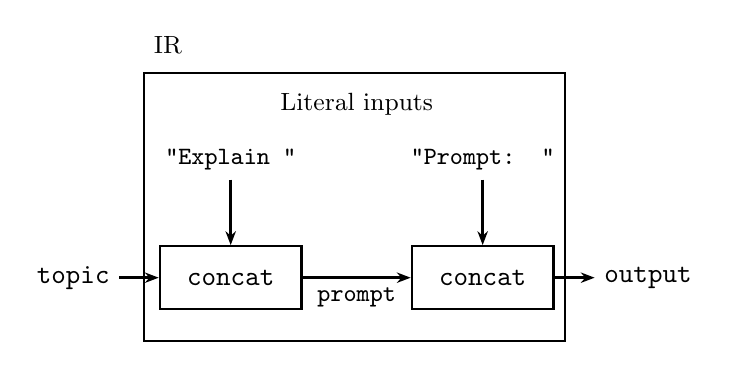
\begin{tikzpicture}
    \irframe{(0.9,-0.8)}{(6.25,2.6)}
    \node[note,anchor=west] at (0.9,2.95) {IR};
    \node (topic) at (0, 0) {\texttt{topic}};
    \node[box] (first) at (2, 0) {\texttt{concat}};
    \node[box] (second) at (5.2, 0) {\texttt{concat}};
    \node (output) at (7.3, 0) {\texttt{output}};
    \node[note] (explain) at (2, 1.5) {\texttt{"Explain "}};
    \node[note] (prefix) at (5.2, 1.5) {\texttt{"Prompt: "}};

    \draw[flow] (topic) -- (first);
    \draw[flow] (first) -- node[below, note] {\texttt{prompt}} (second);
    \draw[flow] (second) -- (output);
    \draw[flow] (explain) -- (first);
    \draw[flow] (prefix) -- (second);
    \node[note] at (3.6, 2.2) {Literal inputs};
\end{tikzpicture}
\end{document}
